\documentclass[border=4pt]{standalone}
\usepackage{fontspec}
\setmainfont{Times New Roman}
\setmonofont{Consolas}
\usepackage{tikz}
\usetikzlibrary{arrows.meta,positioning,shapes.geometric,calc}
\definecolor{tutorteal}{HTML}{087F7A}
\definecolor{tutorlight}{HTML}{EDF7F5}
\definecolor{tutorink}{HTML}{20323C}
\newcommand{\code}[1]{\texttt{\detokenize{#1}}}
\tikzset{box/.style={draw=tutorteal,rounded corners=2pt,fill=tutorlight,
 align=center,minimum height=10mm,text width=35mm,font=\small,inner sep=5pt},
 decision/.style={diamond,aspect=2.0,draw=tutorteal,fill=white,align=center,
 text width=23mm,font=\small,inner sep=1pt},
 flow/.style={-{Latex[length=2mm]},thick,draw=tutorink},
 optional/.style={flow,dashed}}
\begin{document}
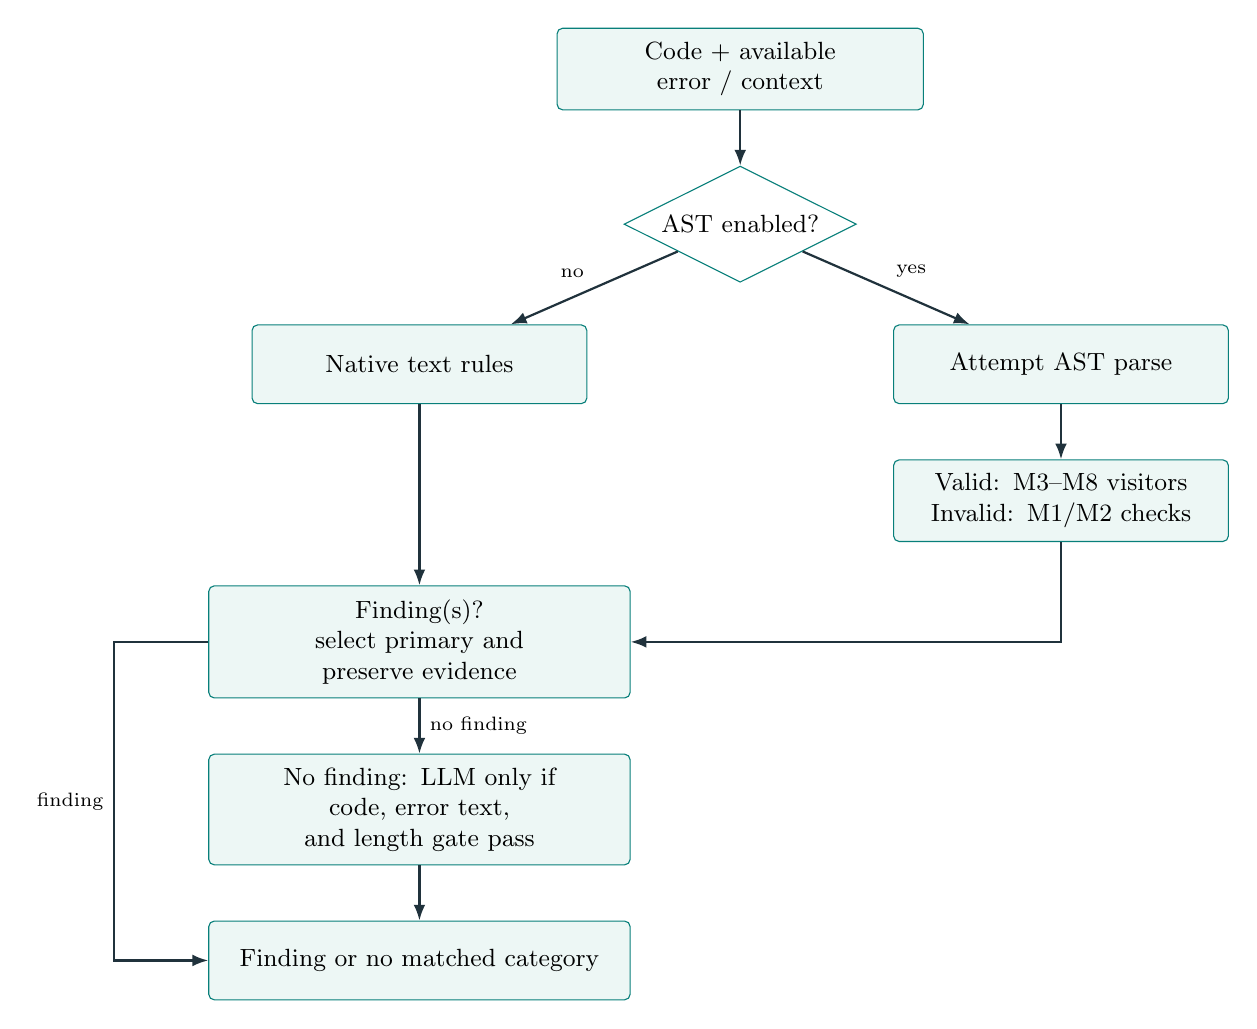
\begin{tikzpicture}[node distance=7mm and 20mm]
\node[box,text width=43mm] (input) {Code + available error / context};
\node[decision,below=of input] (flag) {AST enabled?};
\node[box,text width=39mm,below left=9mm and 12mm of flag] (regex) {Native text rules};
\node[box,text width=39mm,below right=9mm and 12mm of flag] (parse) {Attempt AST parse};
\node[box,text width=39mm,below=of parse] (checks) {Valid: M3--M8 visitors\\Invalid: M1/M2 checks};
\node[box,text width=50mm,below=23mm of regex] (found) {Finding(s)?\\select primary and preserve evidence};
\node[box,text width=50mm,below=of found] (fallback) {No finding: LLM only if\\code, error text, and length gate pass};
\node[box,text width=50mm,below=of fallback] (output) {Finding or no matched category};
\draw[flow] (input)--(flag);
\draw[flow] (flag)--node[above left,font=\scriptsize]{no}(regex);
\draw[flow] (flag)--node[above right,font=\scriptsize]{yes}(parse);
\draw[flow] (parse)--(checks);
\draw[flow] (regex)--(found);
\draw[flow] (checks.south) |- (found.east);
\draw[flow] (found)--node[right,font=\scriptsize]{no finding}(fallback);
\draw[flow] (fallback)--(output);
\draw[flow] (found.west)--++(-12mm,0) |- node[pos=0.25,left,font=\scriptsize]{finding}(output.west);
\end{tikzpicture}
\end{document}
